\documentclass[]{article}
\usepackage[pdftex]{graphicx}
\usepackage[top=1in, bottom=1in, right=1.25in, left=1.25in]{geometry}
\usepackage{hyperref}
\hypersetup{colorlinks=true, linkcolor=blue, urlcolor=blue}

\begin{document}
	\tableofcontents
	\newpage
	
	
	% Fifth Entry
	\section{Group Meeting with Clients 09/12/2012}
		\subsection{Base System Requirements}
			\begin{itemize}
				\item Images must be easy to transfer to the student
					\subitem Could be sent via email, through a link inviting them to view a different site, net space, etc.
				\item Professor must be able to review the images before okay-ing them for distribution.
					\subitem Must be able to select different ‘key’ images if they want.
				\item Must be able to enlarge/interact with and edit after export
				\item System should not need to be plugged in
				\item Set up can be longer the first time as long as you can save the settings so that it doesn’t take so long in the future.
					\subitem Setup vs. Calibration
					\subitem Active time vs inactive time
						\subsubitem It can take longer to set up if it doesn’t need constant attention. Inactive time to set up is much better than active time.
					\subitem 5 min reasonable
				\item Time stamps of when erasing happens
					\subitem Goal 1: End product
					\subitem Goal 2: Step by step board
			\end{itemize}
	
	
	% Fourth Entry
	\section{Individual Work on Further Research and Website Content 09/12/2012}
		\subsection{Website Content}
			\begin{itemize}
				\item Added calendars to both the front page and our meetings page.
				\item Created new ProPANE calendar
				\item Added Griffin's Calendar and ProPANE's calendar to website calendar
			\end{itemize}
		\subsection{Further Research}
			Found a page that seems to have a piece of demo software available to those with access to Microsoft Research’s internal website:\\
			http://research.microsoft.com/en-us/um/people/zhang/WhiteboardIt/\\
			This system takes an image and filters out key information.
			
			The software and technology as a whole is still in its research/development stages. It is a joint project with MS Research and MS Hardware called Distributed Meetings. They have a few technologies going together: A 360 degree video and audio recorder, a Whiteboard image capturing system, (most relevant to us) a PC graphics capture system. Their idea is to record the meeting in several different ways, and then provide easily accessible ways to view all meeting content.
		
			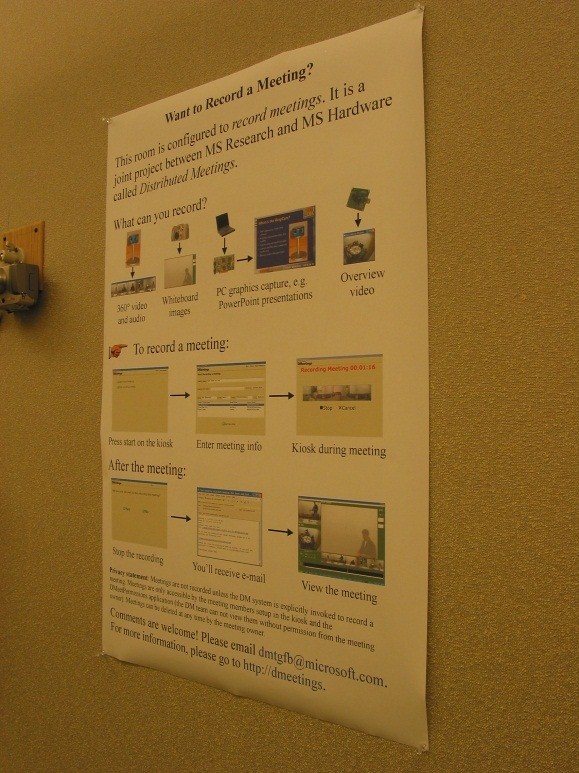
\includegraphics{images/WhiteboardIt.jpg}
			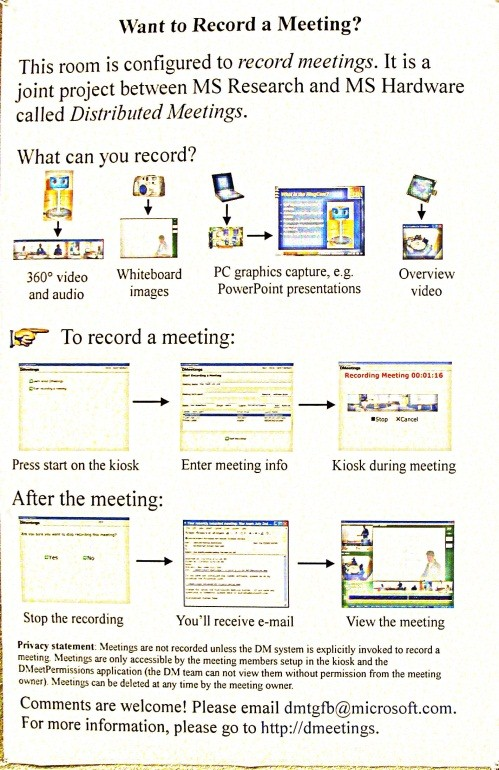
\includegraphics{images/WhiteboardIt2.jpg}\\
			
			We may wish to contact dmtgfb@microsoft.com to ask for more information on their image processing algorithms later on in the process.\\
			\\
			I’m not sure how helpful this might be, but here is a link to Ink-Enabled Apps For Tablet PC\\
			http://msdn.microsoft.com/en-us/magazine/cc967278.aspx\\
			\\
			http://www.fxpal.com/?p=reboard\\
			http://arxiv.org/abs/0911.0039\\
			The following is a paper that talk about another whiteboard captureing technology called ReBoard:\\
			http://arxiv.org/ftp/arxiv/papers/0911/0911.0039.pdf\\
			http://www.fxpal.com/publications/FXPAL-PR-10-546.pdf\\
			
		\subsection{Additional Apps:}
			\begin{itemize}
				\item Whiteboard Capture
				\item Whiteboard Share
				\item WBConference
				\item Whiteboard Snap
				\item BoardTable
			\end{itemize}

	
	% Third Entry
	\section{09/11/2012}
		I first uploaded pictures to the website for our personal biographies.
		\\
		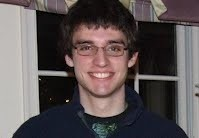
\includegraphics{images/Griffin.jpg}
		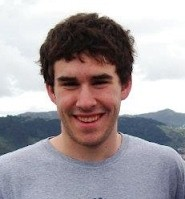
\includegraphics{images/Colin.jpg}
		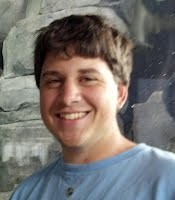
\includegraphics{images/Phil.jpg}
		\\
					After this I wrote an overview about ProPANE on our front page:\\
			Welcome to the website for the Electrical and Computer Engineering senior design project led by Griffin Dunn, Phil Stahlfeld, and Colin Madigan.
			ProPANE's goal is to design and implement a system that will automatically capture all information written on a board during class. This system will then present the saved information in a readily accessible manner so that Bucknell can both better meet the needs of students with disabilities and provide professors with a means to easily compare their notes with the actual information presented in a lecture.
			This project was motivated by Bucknell’s desire to cheaply meet the needs of their students with disabilities. Hiring professional note takers is an expensive endeavor and finding cheaper alternatives is much more desirable.
			This project involves the capture of information from a 2D surface. It will likely require image capture and image processing technology.
		\subsection{Design Constraints}
			\begin{itemize}			
				\item ProPANE must be fully autonomous. After setup the system should require little to no outside interference. The professor should be able to turn it on and leave it running during class and afterwards return to find a set of images depicting everything that was on the board during class.
				\item The information must be presented in a format that allows for easy manipulation, zooming, and editing so that students with disabilities can easily view all content that is displayed on the board.
				\item The system must be discreet. It cannot make loud noises, flashes of light, or create any other forms of distraction during class. Students must be able to concentrate on the lecture not the board capture device.
			\end{itemize}

	
	
	% Second Entry
	\section{Individual Work on Competing Technologies 09/05/2012}
		We have three technologies to compete with: 
		
		\subsection{The Phone App}
			There are several smartphone apps out there that will scan pictures of white boards and filter out the unnecessary information. These applications range from free to a couple dollars on most app stores.\\
				http://www.beetlebugsoftware.com/ is a good example. \\

				Other notable apps:
					\begin{itemize}
						\item Qipit White
						\item Genius Scan
						\item JotNot Scanner Pro
						\item Whiteboard Capture Pro
					\end{itemize}

			However, this IS an issue because it is an area that could possibly pose legal problems. If the resolution is too poor, then the system would be giving ProPANE reliant students a disadvantage. In my opinion, that would be a complete failure of the project.\\
			
		\subsection{Scanners}
			There are scanners that you can attach to an existing white board. After calibrating these scanners, they track your movements using the combination of the sanner and an electronic pen. These electronic pens have replaceable dry erase tips to draw with and replaceable batteries to keep them charged. Some of them require a projector to display background information and others do not.\\

			Examples:
				\begin{itemize}
					\item MimoCapture
					\item eBeam System 3
					\item Interlink FreeBeam
				\end{itemize}

			
		\subsubsection{Electronic Whiteboards}
			Electronic whiteboards are special boards that sense pressure and can display electronic pen interactions with a high degree of accuracy. These displays come in two standard varieties: Those that are electronic displays and those that require a projector to project both the images and any user-inputted writing. Electronic whiteboards tend to be the easiest to use, but they're not very portable because the entire board is required. The trade-off for poor portability is that they can do much more. Multiple people can interact with the board at the same time, and it can be a much more interactive experience. \\

			Examples:
			\begin{itemize}
				\item Smarttech’s SMARTboard 
				\item Panasonic’s Panaboard 
				\item Hitachi’s Starboard 
				\item The Promethean board 
			\end{itemize}

	
	%First Entry
	\section{Initial Group Meeting 08/30/2012}
			\emph{With Phil Stahlfeld and Colin Madigan}\\
			
			Began working on group tasks:
			\begin{itemize}
				\item Team Name
				\item Team Logo
				\item Document Template
				\item Design Specifications
			\end{itemize}
			
		\subsection{Team Name}
			After some discussion we decided that names such as ‘White board scanner’ and ‘board capture system’ weren’t catchy enough. We decided to create an acronym instead so to make our name catchier and thus more memorable. Colin finally came up with our final acronym: ProPANE, short for Professional Portable Automatic Note Extractor. With this agreed upon we moved on to deciding upon our team logo. \\

		\subsection{Team Logo}
			We decided that our logo had to relate to our team name, so with that in mind we searched for images related to the molecular structure of propane. Our favorite image is shown below, and has been adopted as our team logo:\\
			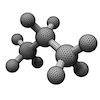
\includegraphics{images/logo.jpeg}\\

		\subsection{Document Template}
			We decided to use LaTEX as our default layout manager for all of our documents. We chose this formatter because it takes care of all the formatting and leaves us with the job of finding and preparing the information, which is the more important part of our job. 

		\subsection{Technical Specifications}
			As noted in our first deliverable, “The goal of this project is to create a system that captures all of the information written on a board during a class in a readily accessible manner. The two driving forces behind solving this problem are: autonomous collection of notes for students with disabilities and providing a means for professors to compare their notes with the actual information presented during a lecture.” \\

			We will be meeting with Robert Midkiff and Douglas Gabauer on 09/13/2013 to discuss more detailed specifications for the project.\\

		
	
	
\end{document}